%%%%%%%%%%%%%%%%%%%%%%%%%%%%%%%%%%%%%%%%%
% Journal Article
% LaTeX Template
% Version 2.0 (February 7, 2023)
%
% This template originates from:
% https://www.LaTeXTemplates.com
%
% Author:
% Vel (vel@latextemplates.com)
%
% License:
% CC BY-NC-SA 4.0 (https://creativecommons.org/licenses/by-nc-sa/4.0/)
%
% NOTE: The bibliography needs to be compiled using the biber engine.
%
%%%%%%%%%%%%%%%%%%%%%%%%%%%%%%%%%%%%%%%%%

%----------------------------------------------------------------------------------------
%	PACKAGES AND OTHER DOCUMENT CONFIGURATIONS
%----------------------------------------------------------------------------------------

\documentclass[
	a4paper, % Paper size, use either a4paper or letterpaper
	10pt, % Default font size, can also use 11pt or 12pt, although this is not recommended
	unnumberedsections, % Comment to enable section numbering
	twoside, % Two side traditional mode where headers and footers change between odd and even pages, comment this option to make them fixed
]{LTJournalArticle}

\usepackage{paralist}

\addbibresource{sample.bib} % BibLaTeX bibliography file

\runninghead{Understanding the Amazon from space} % A shortened article title to appear in the running head, leave this command empty for no running head

\footertext{Deep Learning with Tensorflow, spring 2023} % Text to appear in the footer, leave this command empty for no footer text

\setcounter{page}{1} % The page number of the first page, set this to a higher number if the article is to be part of an issue or larger work

%----------------------------------------------------------------------------------------
%	TITLE SECTION
%----------------------------------------------------------------------------------------

\title{Understanding the Amazon from space} % Article title, use manual lines breaks (\\) to beautify the layout

% Authors are listed in a comma-separated list with superscript numbers indicating affiliations
% \thanks{} is used for any text that should be placed in a footnote on the first page, such as the corresponding author's email, journal acceptance dates, a copyright/license notice, keywords, etc
\author{%
	Bozhidar Ivanov, Emil Yordanov and Kaloyan Kutiyski
}

% Affiliations are output in the \date{} command


% Full-width abstract
\renewcommand{\maketitlehookd}{%
	\begin{abstract}
		\noindent Deforestation in the Amazon Basin has severe consequences on biodiversity, habitat loss, climate change, and other devastating effects. Timely and accurate monitoring of deforestation is critical for effective response. In this research, we propose a solution to the Planet dataset challenge, which involves classifying satellite images to identify deforestation and the types of land cover and use. We experimented with both custom and pre-trained  convolutional neural networks (CNN) trained on the Planet dataset, leveraging their ability to learn spatial patterns on images and reached sufficiently high accuracy for the model to be useful for detecting deforestation
	\end{abstract}
}

%----------------------------------------------------------------------------------------

\begin{document}

\maketitle % Output the title section

%----------------------------------------------------------------------------------------
%	ARTICLE CONTENTS
%----------------------------------------------------------------------------------------

\section{Introduction}

Deforestation in the Amazon Basin accounts for a significant loss of forest cover, contributing to reduced biodiversity, habitat loss, climate change, and other devastating effects. Accurate monitoring of deforestation and understanding its causes and patterns is crucial for effective response and conservation efforts. The availability of high resolution satellite imagery, such as the Planet dataset, presents an opportunity to leverage machine learning techniques for automated deforestation detection and land cover and land use classification.



When solving satellite image classification problems, it’s common to rely on convolutional neural networks. One of the benefits is that we can use an existing CNN with either no modification at all or with retraining some of the final layers and have a powerful feature extraction layer. On top of the CNN a shallow neural network or even an XG Boosted decision can classify chips with accuracy percentage in the high eighties to low nineties.

%------------------------------------------------

\section{Dataset}

\href{https://www.kaggle.com/competitions/planet-understanding-the-amazon-from-space/data}{The Planet dataset} is based on pictures of the Amazon basin taken by the Flock 2 geostationary orbit satellite. Each image was then split into 256x256 pixel ‘chips’ for ease of use by machine learning algorithms, then each of these chips is labeled with each of the seventeen classes of land use specified by the Planet team.

Each chip in the dataset corresponds to an area of 89.72 hectares (947 by 947 meters). The training and test datasets contain 40,799 and 40,669 images each. While at its raw state the dataset contained over 150,000 images, the Planet team chose to discard some of them and crowdsourced the labelling of the rest. 

\begin{figure} 
	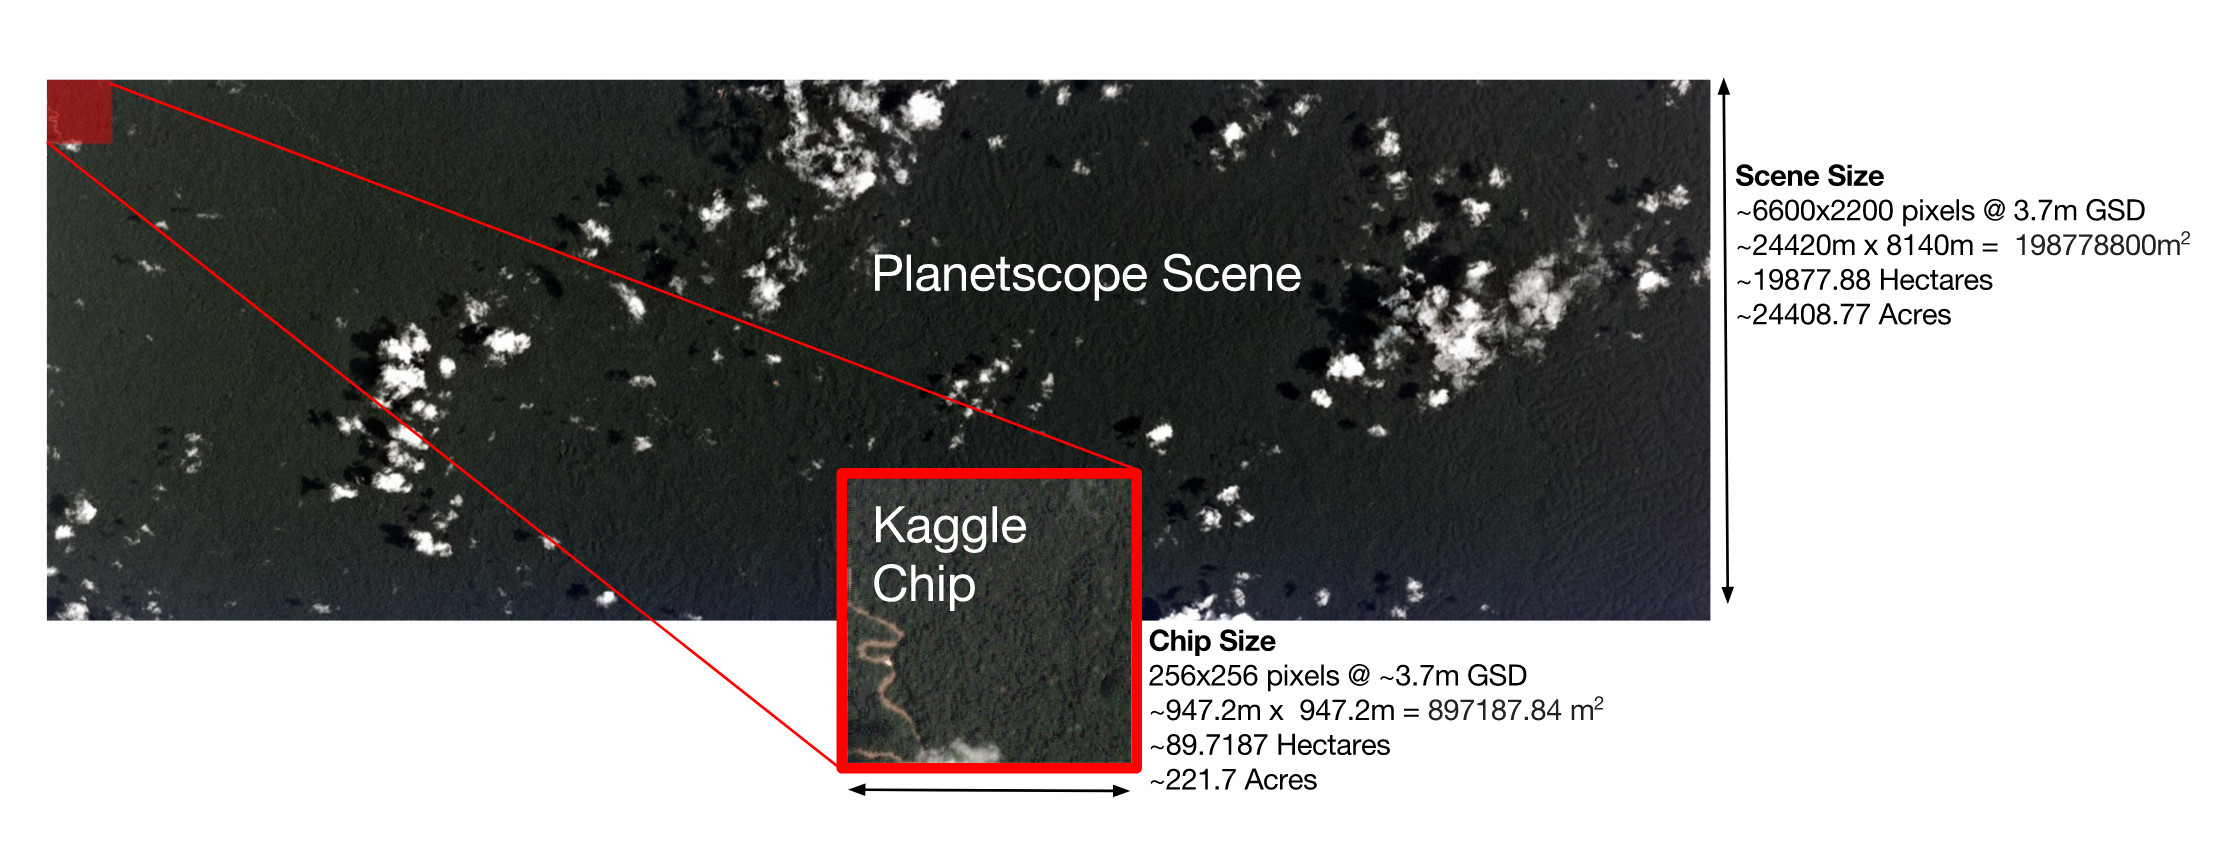
\includegraphics[width=\linewidth]{Figures/chipdesc.jpg}
	\caption{Examples of a chip extracted from a larger satellite image \href{https://storage.googleapis.com/kaggle-competitions/kaggle/6322/media/chips.jpg}{}}
	\label{fig:tcanther}
\end{figure}

Of the 17 types of land use that the model should recognise four refer to the level of cloud cover in the image:
\[\begin{inparaitem}
	\item 'clear'
	\item 'haze'
	\item ‘partly cloudy’
    \item ‘cloudy’
\end{inparaitem}\]
Every image has been labeled with one of these, as it is quite important to be able to gauge the visibility over any specific place - any good well trained model should be able to recognize that the scene is too cloudy to classify anything underneath.

Another six (with ‘primary’ referring to jungle), represent the bulk of land use, and are as such rather common:
\[\begin{inparaitem}
	\item 'agriculture'
	\item 'bare\_ground'
	\item ‘cultivation
\end{inparaitem}\]
 \[\begin{inparaitem}
    \item ‘habitation’
    \item ‘primary’
    \item ‘water’
\end{inparaitem}\]

The following four refer to more specific and more rarely observed types of land use.
\[\begin{inparaitem}
	\item 'artisinal\_mine'
	\item 'conventional\_mine'
 \end{inparaitem}\]
 \[\begin{inparaitem}
	\item ‘selective\_logging'
	\item ‘slash\_burn'
\end{inparaitem}\]
Selective logging is obviously preferable over full on land clearane, while slash and burn agriculture is potentially much more destructive than standard agriculture.

The last two labels are for peculiar and transient natural phenomena - large concentrations of blooming plants and sections of forest flattened by high speed winds.
\[\begin{inparaitem}
	\item 'blooming'
	\item 'blow\_down'
\end{inparaitem}\]

As such the dataset is rather unbalanced in favor of some classes over others. However even the capability to differentiate between natural cover and land use by humans can be useful for a deforestation focused application.

\begin{figure} 
	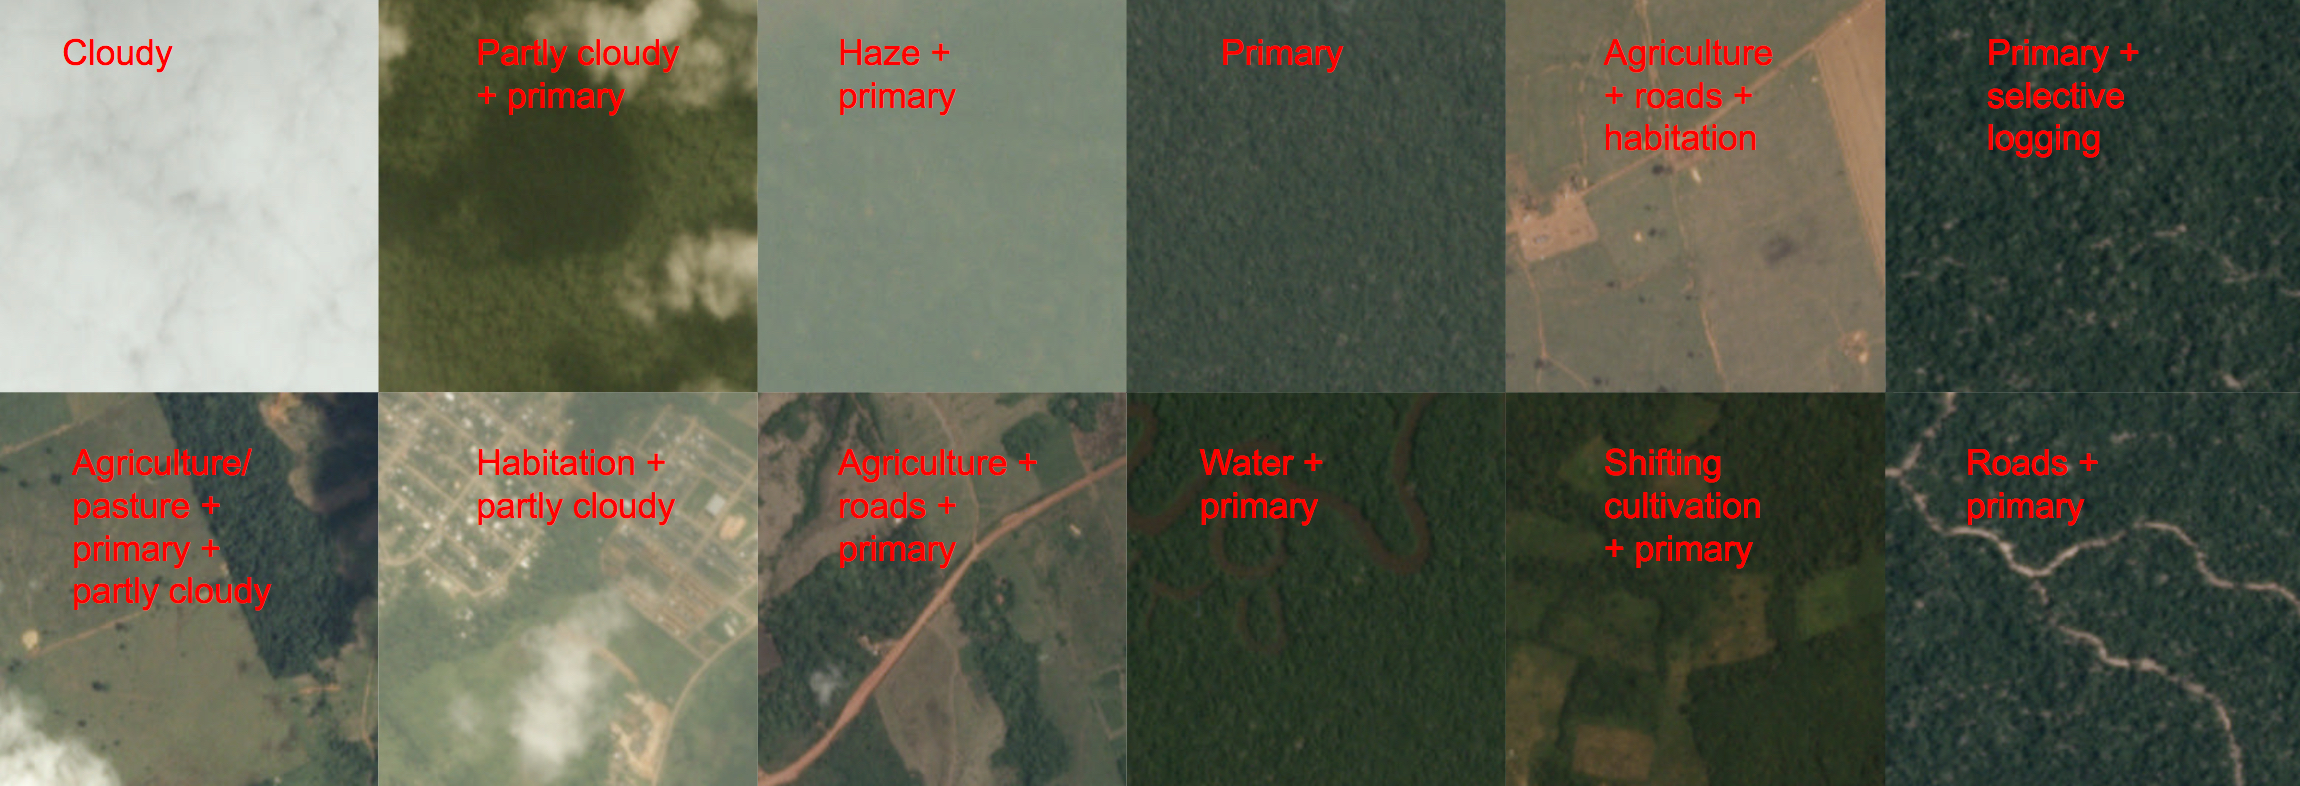
\includegraphics[width=\linewidth]{Figures/chips.jpg}
	\caption{Examples of chips, \href{https://storage.googleapis.com/kaggle-competitions/kaggle/6322/media/chips.jpg}{}.}
	\label{fig:tcanther}
\end{figure}

\section{Training}

\subsection{Data Augmentation}

\subsection{Custom Model}

The large number of images on which the model is trained should ensure significant defense against overtraining, however we also applied some image preprocessing techniques via the standard Keras image preprocessing package.

\begin{verbatim}
train_datagen = ImageDataGenerator(
    rescale=1./255,
    horizontal_flip=True,
    vertical_flip=True,
    rotation_range=40,
    zoom_range=0.2,
    shear_range=0.2)
\end{verbatim}

Using the the following convolutional network we achieved 60\% accuracy after training for 30 epochs. The model uses a sequence of traditional 2D convolution layers and pooling layers sandwiched in between.

\begin{verbatim}
model = tf.keras.models.Sequential([
    tf.keras.layers.Conv2D(
        32, (3, 3), 
        activation = 'relu', 
        input_shape = (
            image_size[0], 
            image_size[1], 3)),
    tf.keras.layers.MaxPooling2D(2, 2),
    tf.keras.layers.Conv2D(
    64, (3, 3), 
        activation='relu'),
    tf.keras.layers.MaxPooling2D(2, 2),
    tf.keras.layers.Conv2D(
        128, (3, 3), 
        activation = 'relu'),
    tf.keras.layers.MaxPooling2D(2, 2),
    tf.keras.layers.Conv2D(
        128, (3, 3), 
        activation = 'relu'),
    tf.keras.layers.MaxPooling2D(2, 2),
    tf.keras.layers.Flatten(),
    tf.keras.layers.Dense(
        512, 
        activation = 'relu'),
    tf.keras.layers.Dense(
        num_classes, 
        activation = 'sigmoid')
])
\end{verbatim}

Additionally, we wanted to evaluate the capabilities of at least one existing neural network, and since it has been observed that Efficient Net can classify images or retrain its top layer using less computing power than other CNNs, while also losing little to no accuracy, we also experimented with efficient net and observed significantly higher accuracy - 90\%, proving, as we had expected, that large pre-trained CNNs are quite adept at solving this type of problem.
%------------------------------------------------


%----------------------------------------------------------------------------------------
%	 REFERENCES
%----------------------------------------------------------------------------------------

\section{Resources}

\begin{enumerate}
    \item While working on this project the following repository and the linked articles were especially useful, but none were quoted directly: \href{https://github.com/satellite-image-deep-learning/techniques#1-classification}{Techniques for deep learning on satellite and aerial imagery}

    \item The overview of the problem and datasets by Planet was also crucial: \href{https://www.kaggle.com/competitions/planet-understanding-the-amazon-from-space/overview}{Planet: Understanding the Amazon from Space}
\end{enumerate}
 
\printbibliography % Output the bibliography

%----------------------------------------------------------------------------------------

\end{document}
